\documentclass[sigconf,nonacm]{acmart}
\usepackage{amsmath,booktabs,tabularx,xurl}
\emergencystretch=2em
\clubpenalty=10000
\widowpenalty=10000
\displaywidowpenalty=10000
\brokenpenalty=10000
\hyphenation{co-activity Listen-Brainz counter-factual PHAN-TOM}
\settopmatter{printacmref=false,printfolios=true}
\setcopyright{none}
\AtBeginEnvironment{thebibliography}{\interlinepenalty=10000}
\newcommand{\scope}{\textit{controlled planted-coordination benchmark}}
\title[PHANTOM: Benchmark Validity and Causal Limits]{PHANTOM: Benchmark Validity and Causal Limits in Coordinated Listening}
\subtitle{NEXUS Research Initiative · Independent Technical Report · October 2026}
\author{Nischit Girish Kumar}
\affiliation{\institution{NEXUS Research Initiative --- Independent Research}\country{}}
\renewcommand{\shortauthors}{Nischit Girish Kumar}
\begin{document}
\begin{abstract}
Coordination detectors are often evaluated on planted patterns, although a successful intervention label does not identify the cause of observed coordination. PHANTOM examines three distinct requirements: benchmark validity, transferable structural evidence, and causal identifiability. An audit of 704.7 million Deezer listening events led to the rejection of benchmarks with origin, catalog and duplicate shortcuts. Matched, structure-preserving interventions and a local permutation reference model then supported controlled external validation on 4,032 ListenBrainz listeners. After the scientific system and manuscript were frozen, a prospective evaluation on 4,032 listeners and 3,714,102 observed September events achieved mean block and pooled AUC 1.000: 378/378 planted treatments alerted and 0/378 matched controls did. These dependent worlds span 42 source groups and carry constructed labels. Independent replay covered all 756 worlds; after a preserved receipt-serialization failure, a separate forensic verifier confirmed immutable outputs without repeating the scientific evaluation. Historical graph reconstruction achieved member and target F1 approximately 0.9167 on a small internal holdout, but shared-stimulus and shifted-overlap tests defeated broader operating claims. Identical-input causal twins expose incompatible detection and attribution requirements under the event-only observation model. The resulting system preserves structural evidence, support boundaries and unresolved alternatives for investigation. The contribution is an auditable account of where coordination evidence is valid and where its interpretation fails; perfect controlled separation is not real-world fraud accuracy.
\end{abstract}
\keywords{coordinated behavior, listening events, conditional randomization, campaign reconstruction, observational equivalence, investigation systems}
\maketitle
\hypersetup{pdftitle={PHANTOM Conference Manuscript FINAL v1},pdfsubject={FINAL v1; Prospective controlled final confirmed; Independent manuscript; not peer reviewed}}
\noindent\textbf{Scope.} Controlled intervention labels on observed listening histories. The prospective result is for the population detector; reconstruction and investigation have separate historical evidence.

\section{Introduction}
A listening group can produce a highly unusual pattern without revealing why its members acted together. An organized manipulation campaign and a recurring shared stimulus can align the same users, recordings and timestamps. A detector may recognize that alignment correctly while a fraud interpretation remains unsupported. This is also an evaluation problem: a benchmark label can describe an intervention that the method detects, yet say nothing about the intentions of the people whose histories form its background.

PHANTOM examines three boundaries that must be evaluated separately. \emph{Benchmark validity} asks whether a score recovers the intended relation rather than source or processing artifacts. \emph{Structural transfer} asks whether a frozen method retains ranking and threshold behavior on another supported population. \emph{Causal identifiability} asks whether the available observations can distinguish the explanations relevant to an investigator. Passing one boundary does not establish the next.

The evidence makes these distinctions consequential. An audit of 704.7 million listening events exposed representation limits; high-scoring synthetic benchmarks were subsequently rejected for origin, catalog and duplicate shortcuts. Repaired matched interventions preserve declared actor marginals while changing cross-actor alignment. A raw score then ranked treatments perfectly but alerted on 22/180 controls, showing that discrimination did not establish threshold transfer. A conditional local-normalization method transferred under the controlled intervention to an external source and, after freezing, to a prospectively committed population of 42 groups: all 378 treatments alerted and none of 378 matched controls did.

That success has a sharp boundary. The detector requires a restrictive recurring schedule, and the final changes the population rather than the intervention family. Separate historical graph testing recovered member and target sets with F1 approximately 0.9167 on only two holdout blocks. Shared-stimulus controls and shifted overlap defeated the broader operating claim. Identical-input causal twins then showed why stronger event-only scoring cannot universally resolve the missing cause. The resulting system returns inspectable evidence and unresolved alternatives rather than an intent judgment.

\paragraph{Contributions.} First, we document a listening-benchmark development in which admissibility checks rejected attractive scores and motivated collision-safe, marginal-preserving comparisons. Second, we characterize conditional relational detection and duplicate-invariant reconstruction through transfer evidence and explicit failure regions, including a prospective frozen evaluation. Third, we connect a concrete identical-input argument to incompatible operational gates and an ambiguity-preserving investigation contract. The intellectual contribution is this connected empirical account of inference boundaries. Permutation models, robust scaling, group detection and observational equivalence are established ideas. No matched published-method comparison establishes superiority; the data do not provide verified fraud labels, production error rates or measured analyst benefit.

\section{Related work}
\subsection{Coordination is an established structural signal}
CopyCatch uses temporal lockstep behavior~\cite{copycatch}; CatchSync combines unusual connectivity and synchronization~\cite{catchsync}; FRAUDAR studies dense bipartite structure under camouflage~\cite{fraudar}. Behavioral-trace networks~\cite{pacheco} and dynamic coordination communities~\cite{tardelli} extend this line beyond individual anomalies. Tardelli et al. explicitly include benign and emergent coordination, so separating coordination from maliciousness is not new here. PHANTOM's narrower contribution is a listening-specific evaluation record that tests what remains defensible after shortcuts and common-cause failures. These methods were not run as matched baselines.

\subsection{Reference models define what an anomaly means}
Temporal-network randomization specifies preserved constraints~\cite{gauvin}; it does not provide a neutral, assumption-free notion of unusualness. PHANTOM conditions on selected schedules, actor item multisets and fixed background. Its local median/MAD normalization uses established robust scaling~\cite{rousseeuw}; its graph comparison uses the nonzero finite-randomization form~\cite{phipson}. The empirical question is whether this combination transfers in the declared listening construction. Neither these precedents nor a perfect controlled result prove exchangeability or error control for natural common-stimulus activity.

\subsection{Listening labels and benchmark validity}
PISA models repeat-aware listening for recommendation~\cite{pisa}; its associated release~\cite{deezerdata} does not supply verified fraud labels. SAGE treats streaming-fraud negative harvesting in a different contextual and labeling regime~\cite{sage}. PHANTOM instead holds observed histories and declared actor marginals fixed across constructed arms. This removes identified origin and marginal shortcuts, but does not make the intervention representative of every natural campaign. A matched comparative study would require equivalent visible data, admissible tuning populations and common evaluation units; borrowing published scores would answer a different question.

\subsection{Attribution requires additional assumptions or evidence}
Causal identification distinguishes observations from the assumptions needed to interpret them~\cite{pearl}. Shalizi and Thomas show how observational network processes can confound homophily, influence and covariate effects~\cite{shalizi}; their result is not a theorem about PHANTOM, but it makes clear that causal ambiguity in network data is established. PHANTOM supplies a simpler listening-domain identical-input construction and a concrete conflict between reconstruction and common-cause suppression gates. Its contribution is the empirical application and system consequence. Scope and fallibility guidance~\cite{amershi} informs the interface contract; following it does not establish investigator effectiveness.

\section{Data and controlled benchmark}
\subsection{Data scale is not detector scale}
The Deezer audit covers 704,728,520 events, 3,444,027 users and 43,803 observed tracks across March--August 2022. There are 500 event parquet files and one 50,000-row embedding file. All 70,472,852 source sessions have exactly ten records, so session boundaries lack validated behavioral meaning. The source contains 2,435,880 excess exact duplicates, about 0.3456\%; individual effects can be larger than the global rate suggests. Same-second ordering and embedding temporal provenance remain unresolved. The release is associated with the PISA dataset~\cite{deezerdata}.

The development sample has 671,410 rows and 3,252 complete release-relative histories. Full-source auditing is disk-backed; frozen detection and reconstruction use bounded samples. It would be incorrect to claim that the graph system was evaluated simultaneously on 704.7 million events. Neither source supplies verified fraud labels or sufficient duration, device, exposure, referral and organizer context for intent attribution. Deezer redistribution rights were not resolved from the visible release page, and raw data is excluded from the proposed public package.

For external validation, ListenBrainz snapshot 2723 is restricted to 1 May 2022 inclusive through 29 May exclusive. After eligibility and prospective sampling, 4,032 listeners in 42 disjoint groups contribute 4,004,802 original events. The representation contains 1,391,257 recording-MSID keys, not verified distinct audio recordings. Selected histories are complete only within that window. Source observations are real; interventions and labels described next are synthetic.

\section{Making a relational benchmark interpretable}
\subsection{Rejecting high scores with the wrong explanation}
An early simulator created multiple campaign families and difficulty regimes around observed background. Generated actors differed in origin, catalog and session properties. Removing session features did not remove the mismatch: synthetic-neutral alerts were 12.08\% versus 4.79\% for observed background. Because the latter is unlabeled, this is a distribution-shift diagnostic rather than a specificity estimate. Further origin probes rejected relational candidates before their downstream scores could be interpreted.

A paired additive intervention still altered actor marginals. A stronger reassignment preserved per-actor item and timestamp multisets, but initially changed semantic duplicate counts in 20/180 pairs. That preprocessing difference invalidated the benchmark even if a detector separated labels. Collision-safe reassignment then repaired the duplicate invariant. The development record therefore does not promote every intermediate performance improvement into accepted evidence.

For selected actor $u$, let $M_u$ be its item multiset and $T_u$ its timestamp multiset. Treatment/control worlds preserve $M_u$, $T_u$, row counts, identity and declared duplicate properties while changing cross-actor item assignment; background remains fixed. Joint item-time association is allowed to change, so preserving marginals is not a claim that every possible actor feature is invariant. The intervention uses 32 recurring slots and eight observed items repeated four times, with difficulty varying synchronized slots at 32, 24 and 16.

\begin{figure*}[t]\centering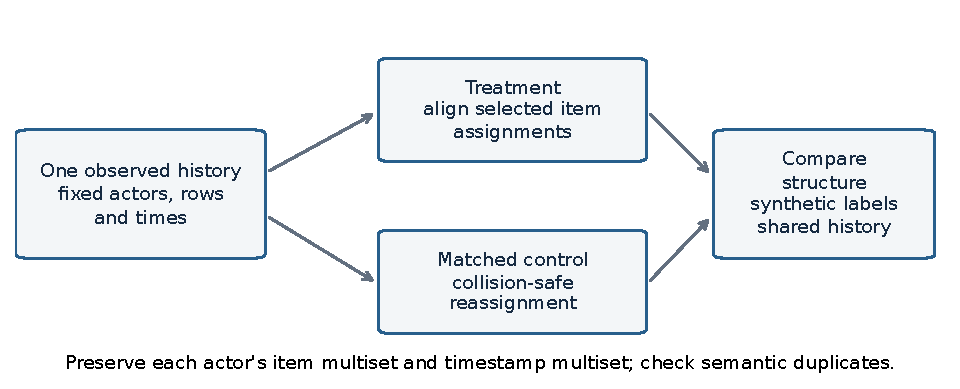
\includegraphics[width=.90\textwidth]{figures/02_counterfactual.pdf}
\caption{Matched controlled worlds preserve declared actor marginals and share source histories. Labels describe the planted intervention, not real participant intent.}
\Description{One observed history branches into an aligned treatment and a collision-safe control, which are compared for relational structure.}\end{figure*}

Whole source blocks and campaigns define evaluation splits. A matched pair is dependent, and several seeds and difficulty levels share a source group. A larger number of constructed worlds is not the same as a larger number of independent populations. Validation remains consumed after use; report preparation does not renew its status.

\subsection{Raw ranking does not imply threshold transfer}
After benchmark repair, a raw relational score achieved perfect ranking in historical validation but alerted on 22/180 controls. Additional global calibration procedures failed per-block alert ceilings: a pooled burden could appear acceptable while a source block failed badly. This distinguishes threshold transfer from discrimination. AUC can remain perfect when both treatment and control scores shift above a threshold.

The accepted response normalizes each eligible world against its own constrained assignment null. This improves transfer in the tested construction by accounting for local baseline and dispersion. It does not remove the need to state the null or show that natural listening satisfies its exchangeability assumptions.

\section{Conditional detection and reconstruction}
\subsection{Population coactivity and a local reference}
For minute bins $b=\lfloor t/60\rfloor$, form unique semantic presences $Q=\{(u,i,b)\}$. Let $n_{ib}$ count actors per item/bin, $N_b$ all actor-item presences per bin, and $d_{ub}$ actor $u$'s distinct items in bin $b$. Population coactivity is
\begin{equation}
C(E)=\frac{\sum_{i,b}n_{ib}(n_{ib}-1)}{\max\{1,\sum_b[N_b(N_b-1)-\sum_u d_{ub}(d_{ub}-1)]\}}.
\end{equation}
Numerator and denominator count ordered cross-actor coincidences and opportunities. The implementation evaluates the full statistic through fixed-background sufficient counts, avoiding repeated materialization of complete null worlds.

The visible selector is narrow: an exact timestamp group has at least eight distinct users each appearing once; the same actor set must recur exactly 32 times in distinct minute bins spanning at least 27 days. Exactly one eligible group is required, otherwise the method is unsupported. This explicit support restriction is essential to interpreting the reported transfer.

Each actor's selected sorted item multiset is independently permuted across its fixed slots, with 4,095 draws and seed 41101. Index randomization draws by $r$. Let $m$ be the median null coactivity and $s=1.4826\operatorname{median}|C^{(r)}-m|$. Robust excess is $Z=(C-m)/s$ when $s>0$, with the frozen alert rule $Z\geq3$. If $s=0$, equality maps to zero and positive/negative deviations to signed $10^{12}$ sentinels. These sentinels are ordering conventions; the score is neither a Gaussian tail probability nor an intent probability.

The null asks whether selected item assignments are exchangeable over the preserved schedule. A shared external stimulus can violate that assumption without intentional manipulation. Detecting a departure is consequently a structural result conditional on the reference model.

\subsection{Duplicate-invariant campaign objects}
Reconstruction starts from unique $(u,i,t)$ atoms in the May window and retains multiplicity descriptively. Canonical ordering uses actor item/time fingerprints; ambiguous fingerprints cause abstention. Selected bursts join consecutive atoms whose gaps are at most 600 seconds. A burst needs at least eight distinct users and eight singleton-user atoms; an actor must participate in at least eight qualifying bursts. After this one-time actor filter, retained groups need two atoms. The procedure does not silently randomize multi-atom cells as if they were singleton observations.

Catalog overlap defines a fixed candidate graph: connect actors sharing at least three selected items and catalog Jaccard at least 0.10, then retain components with at least three actors. Within-actor permutations preserve these catalogs and candidate components. Catalog connectivity alone is not an alert.

For actors $u,v$, count shared selected slots with the same item and same fixed bin at width $h$, giving $w_{uv}^{(h)}$. The component statistic is
\begin{equation}
T(G)=\binom{|G|}{2}^{-1}\sum_{\{u,v\}\subset G}\min(w_{uv}^{(60)},w_{uv}^{(300)}).
\end{equation}
The denominator includes all unordered pairs, including zeros. The 60/300 bins share an origin and are nested: their agreement must not be described as arbitrary time-jitter robustness.

The graph null uses 511 within-actor selected-item permutations, seed 55101. Observed and null component scores receive the same median/MAD normalization. For observed $Z_g$ and null $Z_g^{(r)}$, define $M^{(r)}=\max_g Z_g^{(r)}$ and
\begin{equation}
\widehat p_g=\frac{1+\sum_{r=1}^{511}\mathbf1[M^{(r)}\geq Z_g]}{512}.
\end{equation}
Admission requires $Z_g\geq3$ and $\widehat p_g\leq0.01$. Resolution is $1/512$. The maximum compares a fixed candidate family, but universal familywise calibration for organic listening is not established merely by this construction.

Admitted components link when target Jaccard is at least 0.25 and period overlap at least half the shorter interval. Targets are items shared by two selected member catalogs and may lack direct temporal support. Merged objects retain constituent scores, without an invented merged $p$-value or common-organizer claim. The accepted method is the frozen burst-schedule, consensus, pooled-fragment variant; alternative graph methods are not interchangeable with it.

\subsection{What is evaluated}
AUC describes ranking of constructed labels. Detection and control-alert burden describe the fixed threshold at the world level. Reconstruction uses one-to-one parent/object assignment by member F1; unmatched parents receive zero. Member precision and recall describe matched sets, while target F1 and designated-fragment recovery answer separate questions. Aggregate F1 follows per-parent computation, not the harmonic mean of independently averaged precision and recall. Robustness primary scores retain original truth even when evidence is removed, with surviving-truth analyses reported separately in the historical record.

\paragraph{Output semantics.} A supported non-alert, an unsupported input and withheld attribution are distinct outcomes. Unsupported inputs are not negative classifications. Merged objects preserve constituent evidence; no jointly calibrated merged significance or common-organizer claim is introduced.

\section{Evaluation logic}
Admissibility precedes performance: origin, neutral and duplicate checks determine whether a score answers the intended relational question. Ranking, threshold burden, reconstruction and reviewability then have separate gates. Passing selected perturbations cannot compensate for a failed conjunctive operating requirement. Duplicate defects, a misspecified natural-process null and missing causal information are different failure mechanisms; they do not admit one generic scoring repair.

\section{Evidence and failure boundaries}
\subsection{External population: strong separation, bounded transfer}
The external test freezes the relational detector before applying it to ListenBrainz. Sampling seed 41201 and construction seeds 41211--41213 produce $42\times3\times3=378$ pairs across groups, seeds and difficulties, or 756 worlds. AUC is 1.000, all 378 treatments alert, no matched controls alert, and worst-group control alert rate is zero. These results concern the \scope; real listeners are not assigned real fraud labels.

The historical uncertainty procedure uses 2,000 whole-group bootstrap replicates, seed 41102. Perfect outcomes in every observed group yield degenerate percentile intervals. They describe this empirical distribution, not uncertainty about unseen mechanisms. Disjoint users do not establish independent groups when source periods and construction choices are shared. A zero observed alert count must therefore remain a count, not a claim of zero population error.

External transfer covers the population detector only. It does not validate graph reconstruction, support classification, analyst performance, queue precision or deployment. The intervention remains narrow, and support eligibility is not measured as coverage of an unrestricted production stream.

\begin{table*}[tbp]\centering\small
\caption{Primary evidence by stage. Populations, tasks and denominators are distinct; no overall accuracy score is implied. Final metrics are confirmed from frozen outputs, with the original verifier failure preserved.}
\renewcommand{\arraystretch}{1.18}\begin{tabularx}{\textwidth}{@{}>{\raggedright\arraybackslash}p{.10\textwidth}>{\raggedright\arraybackslash}p{.23\textwidth}>{\raggedright\arraybackslash}p{.16\textwidth}>{\raggedright\arraybackslash}p{.21\textwidth}>{\raggedright\arraybackslash}X@{}}\toprule
Evidence stage & Population & Task & Result & Interpretation limit\\\midrule
Phase 4.12 & May 2022 ListenBrainz; 4,032 listeners; 42 groups; 378 pairs & External controlled detection & AUC 1.000; 378/378 treatments; 0/378 controls & Synthetic intervention labels; consumed external validation.\\
Phase 5.1 & Two historical holdout blocks; 84 pairs; 168 parents & Graph reconstruction & Member/target F1 0.9167; 0/84 controls & Small internal holdout; no external graph validation.\\
Phase 7 & Six reused development blocks; 12 moderate worlds per shock family & Hard-negative robustness & Popularity/release shocks: 12/12 alerts each; shifted-overlap F1 0.3636 & Overall moderate operating region failed.\\
Phase 9.2 & 321 synthetic worlds; 480 candidates; 477 parents & Investigation development & 416/480 candidates reviewable; 327/477 parents covered & Coverage differs by denominator; analyst utility unmeasured.\\
Phase 12 & September 2026 ListenBrainz; 4,032 listeners; 42 groups; 378 pairs & Prospective sealed detection & Block/pooled AUC 1.000; 378/378 treatments; 0/378 controls & Controlled labels; forensic confirmation after receipt failure.\\
\bottomrule\end{tabularx}\label{tab:results}
\end{table*}

\subsection{Reconstruction and why added complexity failed}
Graph development uses six blocks and 252 treatment/control pairs, yielding member F1 0.9067 and 2/252 control alerts for the selected core. The historical internal holdout uses two blocks, 84 pairs and 168 treatment parents. Member precision, recall and F1 and target F1 are each approximately 0.9167; designated-fragment recovery is 1.000; control alerts are 0/84. Exact duplicate perturbations preserve outputs. With only two holdout source blocks, these results do not characterize broad between-population uncertainty.

Earlier graph variants were unacceptable: catalog structure could give attractive F1 while alerting on every control, and initial nulls retained high burden. A behavioral hybrid later reduced actionable member F1 to 0.5357 by vetoing useful structural cases. Non-veto augmentation preserved the core but added zero within-block ranking gain across 210 comparisons. These failures justify retaining a simpler accepted core; they do not show that every possible fusion method is inferior.

\subsection{Separate perturbations and a failed overall envelope}
Historical stress tests reuse the development blocks. Member F1 is 0.7687 under 25\% actor loss, 0.8981 under 25\% event thinning, 0.9167 under 30-second jitter and 0.7540 with a 75\% prefix. A four-disjoint-campaign panel reaches F1 1.000. These are sampled separate settings, not a jointly validated robust operating region.

Shifted 25\% overlap yields member/target F1 0.3636 and full control-world alert burden, unlike simultaneous overlap. Popularity-shock and release-event controls each alert in all 12 moderate worlds. Background absorption reaches 0.2544 in those settings. Routine-listening controls also fail the intended moderate gate. The overall operating-envelope claim is therefore rejected despite several successful perturbations.

\begin{figure*}[t]\centering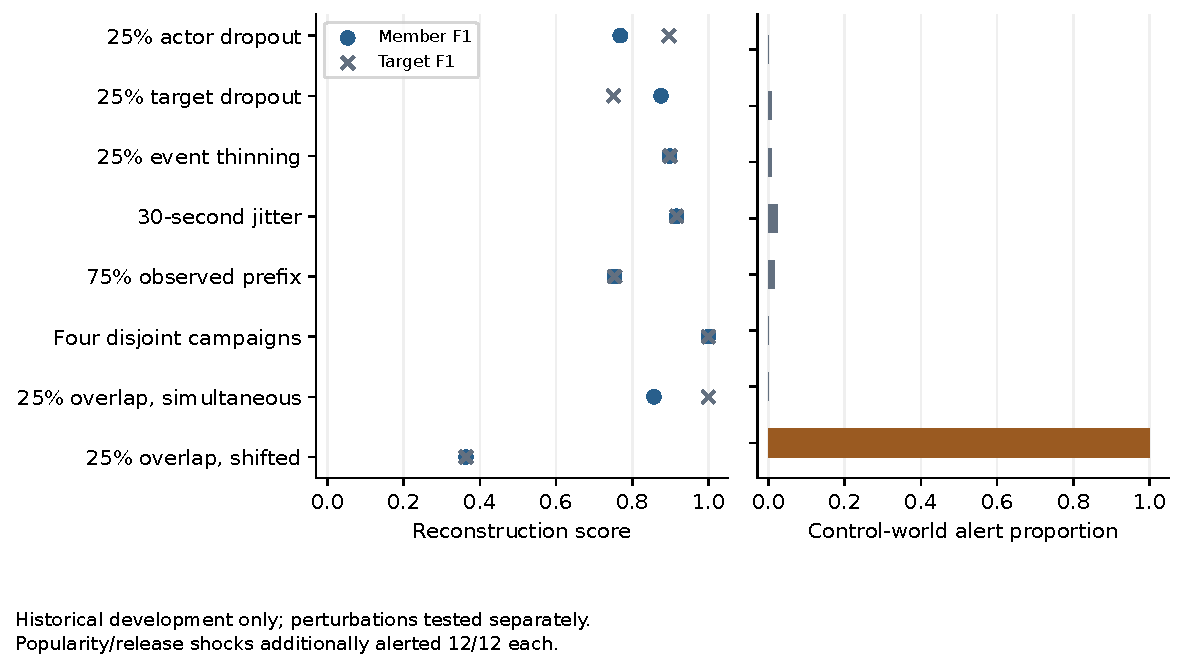
\includegraphics[width=.91\textwidth]{figures/06_robustness.pdf}
\caption{Both moderate successes and a failure region on reused development histories. Plotted aggregates come from frozen reports; no smoothing, new trials or independent-world interpretation is introduced. The additional shock failures prevent a global safe-envelope claim.}
\Description{Member and target F1 remain relatively high for several separate perturbations, but shifted overlap has F1 0.3636 and every control alerts.}\end{figure*}

A shared stimulus may generate genuinely unusual synchronization under the assignment null. Such an alert can be structurally meaningful while failing a manipulation-control requirement. It would be misleading to make the old gate pass by simply renaming the output. Instead, the failure is retained and the governing claim narrowed.

\section{From failed attribution to an investigation contract}
\subsection{An identical-input argument}
Common-cause conditioning suppressed shocks but erased coordinated parents in other fixtures. This motivates an information-level test. Let hidden accounts $H_A$ (intentional coordination) and $H_B$ (recurring external stimulus) yield the same visible array $X=x$. Any deterministic event-only method receives the same input. For randomized $f(X,U)$, with randomness independent of the hidden account,
\begin{equation}
\mathcal L(f(X,U)\mid H_A,X=x)=\mathcal L(f(X,U)\mid H_B,X=x).
\end{equation}
The observation model includes every permitted detector input, and $U$ has the same law under both accounts. The equality follows by integrating $\mathbf1\{f(x,u)\in A\}$ against that common law for any output set $A$. Six causal-twin descriptions instantiate this construction. More powerful features of the same $x$ cannot recover the missing distinction. The result does not imply that all real cases are twins or that external provenance cannot help.

There is also an incompatible-gate consequence. If no alert gives F1 zero and F1 is bounded by one, then $\mathbb E[F1]\leq\Pr(\mathrm{alert})$. A required mean F1 of at least 0.7 on one account implies at least 0.7 alert probability on its identical-input twin, inconsistent with a 0.07 upper alert requirement there. These are constructed requirements, not estimated population rates. The contribution is a clear empirical application of observational equivalence, not a new general theorem about all fraud detection.

\begin{figure*}[t]\centering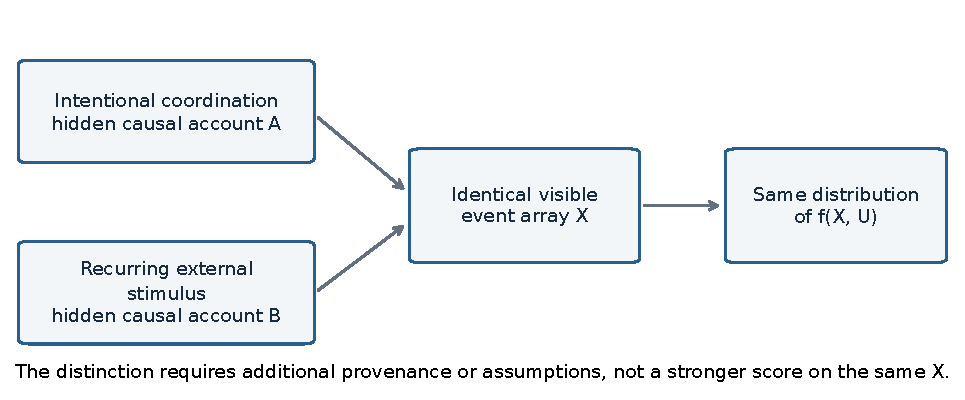
\includegraphics[width=.90\textwidth]{figures/07_causal_twins.pdf}
\caption{Causal twins supply identical visible events under different hidden accounts. Event-only randomness cannot distinguish them when its law is independent of the hidden cause.}
\Description{Intentional coordination and recurring external stimulus lead to the same event array and therefore the same detector output distribution.}\end{figure*}

\subsection{Support, alternatives and equal-priority sets}
PHANTOM consequently separates supported structure from causal interpretation. The operating contract names supported, supported-with-caution, ambiguous-common-cause and out-of-support states. These concern evidence applicability, not fraud probabilities. Event-only attribution remains withheld even for a well-supported structural object. Missing provenance stays explicitly null, and diagnostic objects remain available when interpretation is withheld.

Later defensive testing found identifier-sensitive ranking and unresolved alternatives under bridges and shared responses. A repaired scalar ranking still did not justify a causal preference. The accepted development layer instead uses representation-relative ambiguity-equivalence sets, preserving complete membership and equal scientific priority through display, filtering and export. Display order is nonsemantic. A singleton is not causal certainty, and a set is not proof of a common organizer.

Combined development has 480 candidates across 321 synthetic worlds and 477 original parents. Candidate reviewability is 416/480, whereas original-parent reviewable coverage is 327/477. Expected out-of-support recall remains 40/44. These different denominators must not be substituted. All 230 equivalence classes require provenance. Unseen synthetic fixtures exercise familiar mechanisms, without providing fresh real-population or analyst validation.

\subsection{Inspectable implementation, unmeasured utility}
A read-only dashboard exposes support, constituent evidence, alternatives, lineage and complete equivalence sets on wholly synthetic fixtures. Missing provenance remains explicit, and display order has no scientific meaning. It performs no scientific recomputation or enforcement. The accompanying report describes fidelity checks; neither implementation checks nor a working interface establish analyst effectiveness.

\section{Prospective Sealed Final Evaluation}
\label{sec:final}
\paragraph{Prospective boundary.} The scientific system and PRE-FINAL manuscript were frozen before final population materialization and scoring. The local commitment specified the source, September 1 inclusive--September 29 exclusive 2026 UTC window, exclusions, sampling and construction seeds, detector, metrics and gates. It is not an external registry or third-party timestamp attestation.

Pre-access audit found that the committed \texttt{final412} namespace had no executable mapping. The invalid-before-scoring record was retained. Phase 12A defined a deterministic enrollment/catalog/timestamp mapping, verified it on invented inputs and resealed before final histories were accessed. A later pre-access audit found that execution adapters had been completed after the first lock. Acquisition stopped during archive-header indexing, before event-column access or population selection. Toy/non-final equivalence checks preceded a superseding lock of all final execution bytes. Both locks and the original invalid record remain preserved.

\paragraph{Population and result.} The committed population contains 4,032 listeners in 42 groups of 96 and 3,714,102 original observed events during September 1--28, 2026 UTC. Three construction seeds and three levels yield 378 pairs and 756 worlds. The frozen detector achieved mean block and pooled AUC 1.000, with 378/378 treatment alerts, 0/378 control alerts and 0.0\% worst-block control burden. All 18 applicable scientific gates pass. Figure~\ref{fig:final} shows the group denominators. These are controlled intervention labels on real histories, not verified fraud labels.

The conditional whole-block procedure gives AUC and detection intervals $[1.000,1.000]$, control-mean interval $[0.000,0.000]$ and equal-block upper 95\% control bound 0.0\%. Paired and group dependence remains. Resampling perfect observed groups cannot establish zero natural-population alert probability or performance on unseen mechanisms.

\begin{figure*}[t]\centering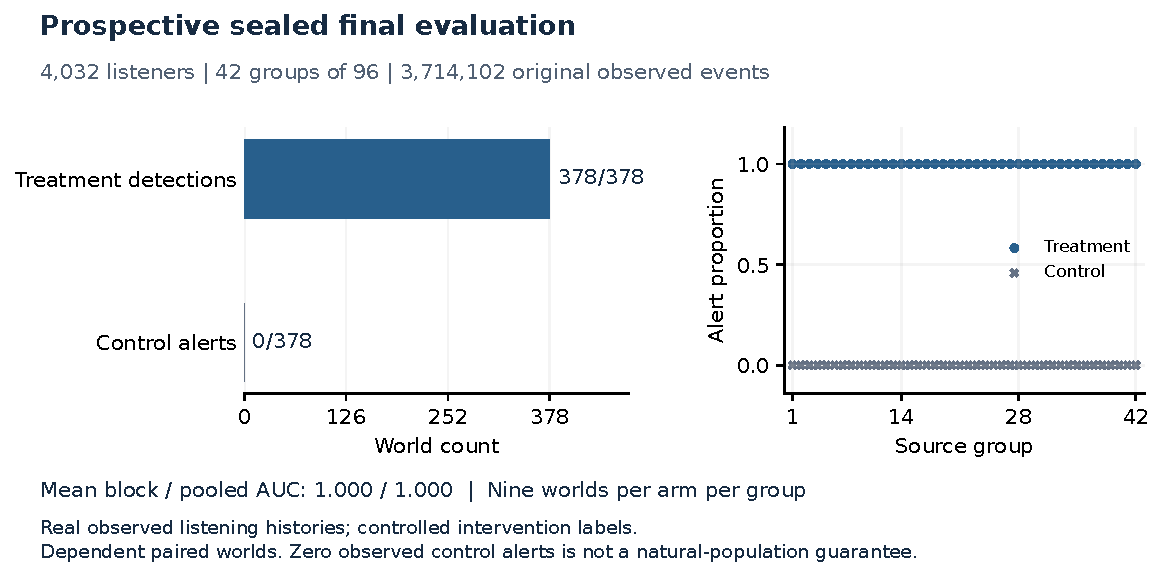
\includegraphics[width=.93\textwidth]{figures/10_prospective_final.pdf}
\caption{Prospective final evaluation: real observed listening histories; controlled intervention labels. Each of 42 groups contributes nine worlds per arm. Perfect separation is conditional on the committed construction and support.}
\Description{All 378 planted treatments alert and none of 378 controls alert; all 42 groups have treatment rate one and control rate zero.}\label{fig:final}\end{figure*}

\paragraph{Verification qualification.} Independent replay covered all 756 worlds. The originally locked verifier then failed during JSON receipt serialization because of a non-scientific NumPy-boolean conversion defect. Its traceback, partial receipt and invalid disposition remain preserved. A separate post-final forensic verifier confirmed every provisional metric exactly and all 18 scientific gates solely from immutable original/replay artifacts. It did not rerun selection, construction, the detector or null generation, or change scientific code, seeds, thresholds or predictions. The canonical scientific evaluation ran once; replay was deterministic verification, not a new scientific trial. Separate forensic-tool initialization and artifact-layout incidents are documented in the supplement. Independent verification denotes implementation/process separation, not institutional verification.

The final supports controlled prospective transfer of the population detector. It does not validate end-to-end graph reconstruction, analyst utility, production behavior or intent attribution. The September population is consumed and cannot become unseen evidence for PHANTOM v2.

\section{Limitations and reproducibility}
\paragraph{Labels and causality (construct validity).} Treatment labels identify planted assignment changes, not dishonest listeners. The event schema omits exposure, referral and organizer provenance. Causal twins demonstrate one exact ambiguity; they do not characterize the prevalence of indistinguishable real cases. Structural significance cannot be reinterpreted as a calibrated probability of intent.

\paragraph{Mechanism and support (external validity).} The exact recurring-schedule selector is aligned with the controlled intervention. Passing invariance checks establishes that the identified shortcuts were addressed, not that the benchmark is generally difficult. Coverage of ordinary streams, unseen coordination mechanisms and natural-process exchangeability remain unknown. The final changes source population and period under the same intervention family.

\paragraph{Dependence and reconstruction (internal and external validity).} The final has 42 source groups, not 756 independent populations. Whole-group resampling retains the observed dependence unit but cannot establish independence across groups or uncertainty over unseen mechanisms. The graph holdout comprises two historical blocks; later stress tests reuse development histories. Prospective detector results do not externally validate reconstruction or investigation coverage.

\paragraph{Comparisons and utility (comparative and operational validity).} No matched published-method baseline establishes superiority. No analyst study, production deployment, enforcement outcome or unrestricted throughput measurement is available. Incomplete parent coverage remains a limitation even when a candidate is reviewable. The dashboard implements an evidence contract; it does not validate its benefit.

\paragraph{Rights and reproducibility (auditability).} Public reproduction covers equations, aggregate figures and wholly synthetic teaching examples. Full experiments require authorized source access; raw histories, protected final truth and uncleared research code are excluded. Local commitments and process-separated verification provide an audit trail, not independent institutional attestation. Detailed seeds, selectors, gates and the complete verification incident are retained in the supplement. Any new comparator experiment or method change requires a separately committed study; the final population is already consumed.

\section{Conclusion}
PHANTOM v1 demonstrates conditional detection of planted coordination across observed listening populations and bounded reconstruction of member and target structure. The prospective final evaluation confirmed perfect separation within its committed controlled procedure; the preserved verifier incident changes the verification history, not the reproduced scientific values. That result does not erase origin confounding, threshold failures, rejected hybrid designs, common-stimulus failures or overlap ambiguity. These findings explain the final task: provide inspectable evidence and investigation priorities while withholding unsupported causal judgments. Matched comparative evaluation, broader support coverage, independent contextual evidence and analyst studies remain future research. Any method change belongs to PHANTOM v2; the consumed September population cannot serve as unseen evidence for it.

\begin{acks}
AI-assisted tools supported selected engineering tasks, with minor assistance in documentation and manuscript preparation. Nischit Girish Kumar directed the research, system architecture, experimental design, validation, and final technical decisions and assumes responsibility for the work. Nischit Girish Kumar is the sole human author; NEXUS Research Initiative denotes independent research.
\end{acks}
\bibliographystyle{ACM-Reference-Format}
\bibliography{references}
\end{document}
